\documentclass[11pt]{article}

\usepackage{comment} % enables the use of multi-line comments (\ifx \fi) 
\usepackage[a4paper,margin=1cm]{geometry}
\usepackage[utf8]{inputenc}
\usepackage[ngerman]{isodate}
\usepackage{gensymb}
\usepackage{graphicx}
\usepackage{booktabs}% http://ctan.org/pkg/booktabs
\usepackage{tabularx}
\usepackage{ltablex} % Longtables with tabularx
\usepackage[x11names]{xcolor}
\usepackage{amsmath}
\usepackage{amssymb}
\usepackage{array}
\usepackage{wrapfig}
\usepackage{subcaption}
\usepackage{csquotes}
\usepackage{lscape}
\usepackage{geometry}
\usepackage{multicol}
\usepackage{bm}
\usepackage{enumitem}
\usepackage{hyperref}
\usepackage{mdframed}
\usepackage{scalerel}
\usepackage{stackengine}
\usepackage{mathtools}
\usepackage{pdfpages}

% Code highlighting
\usepackage{minted}
\surroundwithmdframed{minted}

% Be able to caption equations and float them in place
\usepackage{float}

\newmdtheoremenv{theorem}{Theorem}
\geometry{a4paper, margin=2.4cm}

\newcommand\equalhat{\mathrel{\stackon[1.5pt]{=}{\stretchto{\scalerel*[\widthof{=}]{\wedge}{\rule{1ex}{3ex}}}{0.5ex}}}}
\newcommand\defeq{\mathrel{\overset{\makebox[0pt]{\mbox{\normalfont\tiny def}}}{=}}}
\newcolumntype{C}{>{\centering\arraybackslash}X}

\DeclarePairedDelimiter\abs{\lvert}{\rvert}
\DeclarePairedDelimiter\norm{\lVert}{\rVert}

\setcounter{tocdepth}{3}
\setcounter{secnumdepth}{3}

\graphicspath{{./img/}}

\begin{document}
	
\title{Private Law FS20}
\author{Pascal Baumann\\pascal.baumann@stud.hslu.ch}
\maketitle



For errors or improvement raise an issue or make a pull request on the \href{https://github.com/KilnOfTheSecondFlame/mse_summaries}{github repository}.

\tableofcontents
\newpage



\section{Introduction}
The goal of the module is to foster an understanding on the different dimensions of privacy and a thinking in the corresponding contexts. Transferring privacy aspects to
and within the private and work environment and reflecting upon these, establishing links with learning content in the MRU and the technical modules. Acquiring an appreciation of the legal aspects confronting an engineer in demanding professional situations. Gaining awareness in order to avoid damages due to infringements of rights or legal uncertainty. Acquisition of speaking and listening
skills in order to conduct the corresponding specialist discussions with experts.

Law is a social framework, that saves energy by providing an orientation how to manage conflicts and preserve the values of the culture the law was created in. The law legitimises public authorities and courts, and aims to control the power inherent in any system so that no imbalance is present. 

\subsection{Importance of Law in a Technical or Information Technology World}

The law provides a guideline of the allowed/maximum or obligatory requirement/minimum a system has to satisfy. It clarifies obligations, responsibilities and liability. Industry standards apply the law to a specific field, although they do not clear all legal questions most of the time.

In risk management not only technical or organisational risks have to be considered, but also legal measures to mitigate risks. It is prudent to consult legal as soon as possible in a project, otherwise it may be stopped at the last minute and be very costly. By law, management is responsible that an organisation complies to the legal framework.

\subsection{Importance of Privacy and Personal Data Protection}
Personal data in the wrong hands may harm the person in question in various forms. Privacy and the \emph{right to forget} is essential in personal development. An owner with a big collection of such personal data gets a lot of power with little oversight or control. One of the main tasks of a state is to protect its citizen, this includes protection from attacks on personal data.

\paragraph{One of the Most Vital Legal Questions}
\begin{theorem}
	{\scriptsize (1)} \textbf{Who} wants from {\scriptsize (2)} \textbf{whom} {\scriptsize (3)}\textbf{what} based on what {\scriptsize (4)}\textbf{title} or right?
\end{theorem}

\begin{figure}[H]
	\centering
	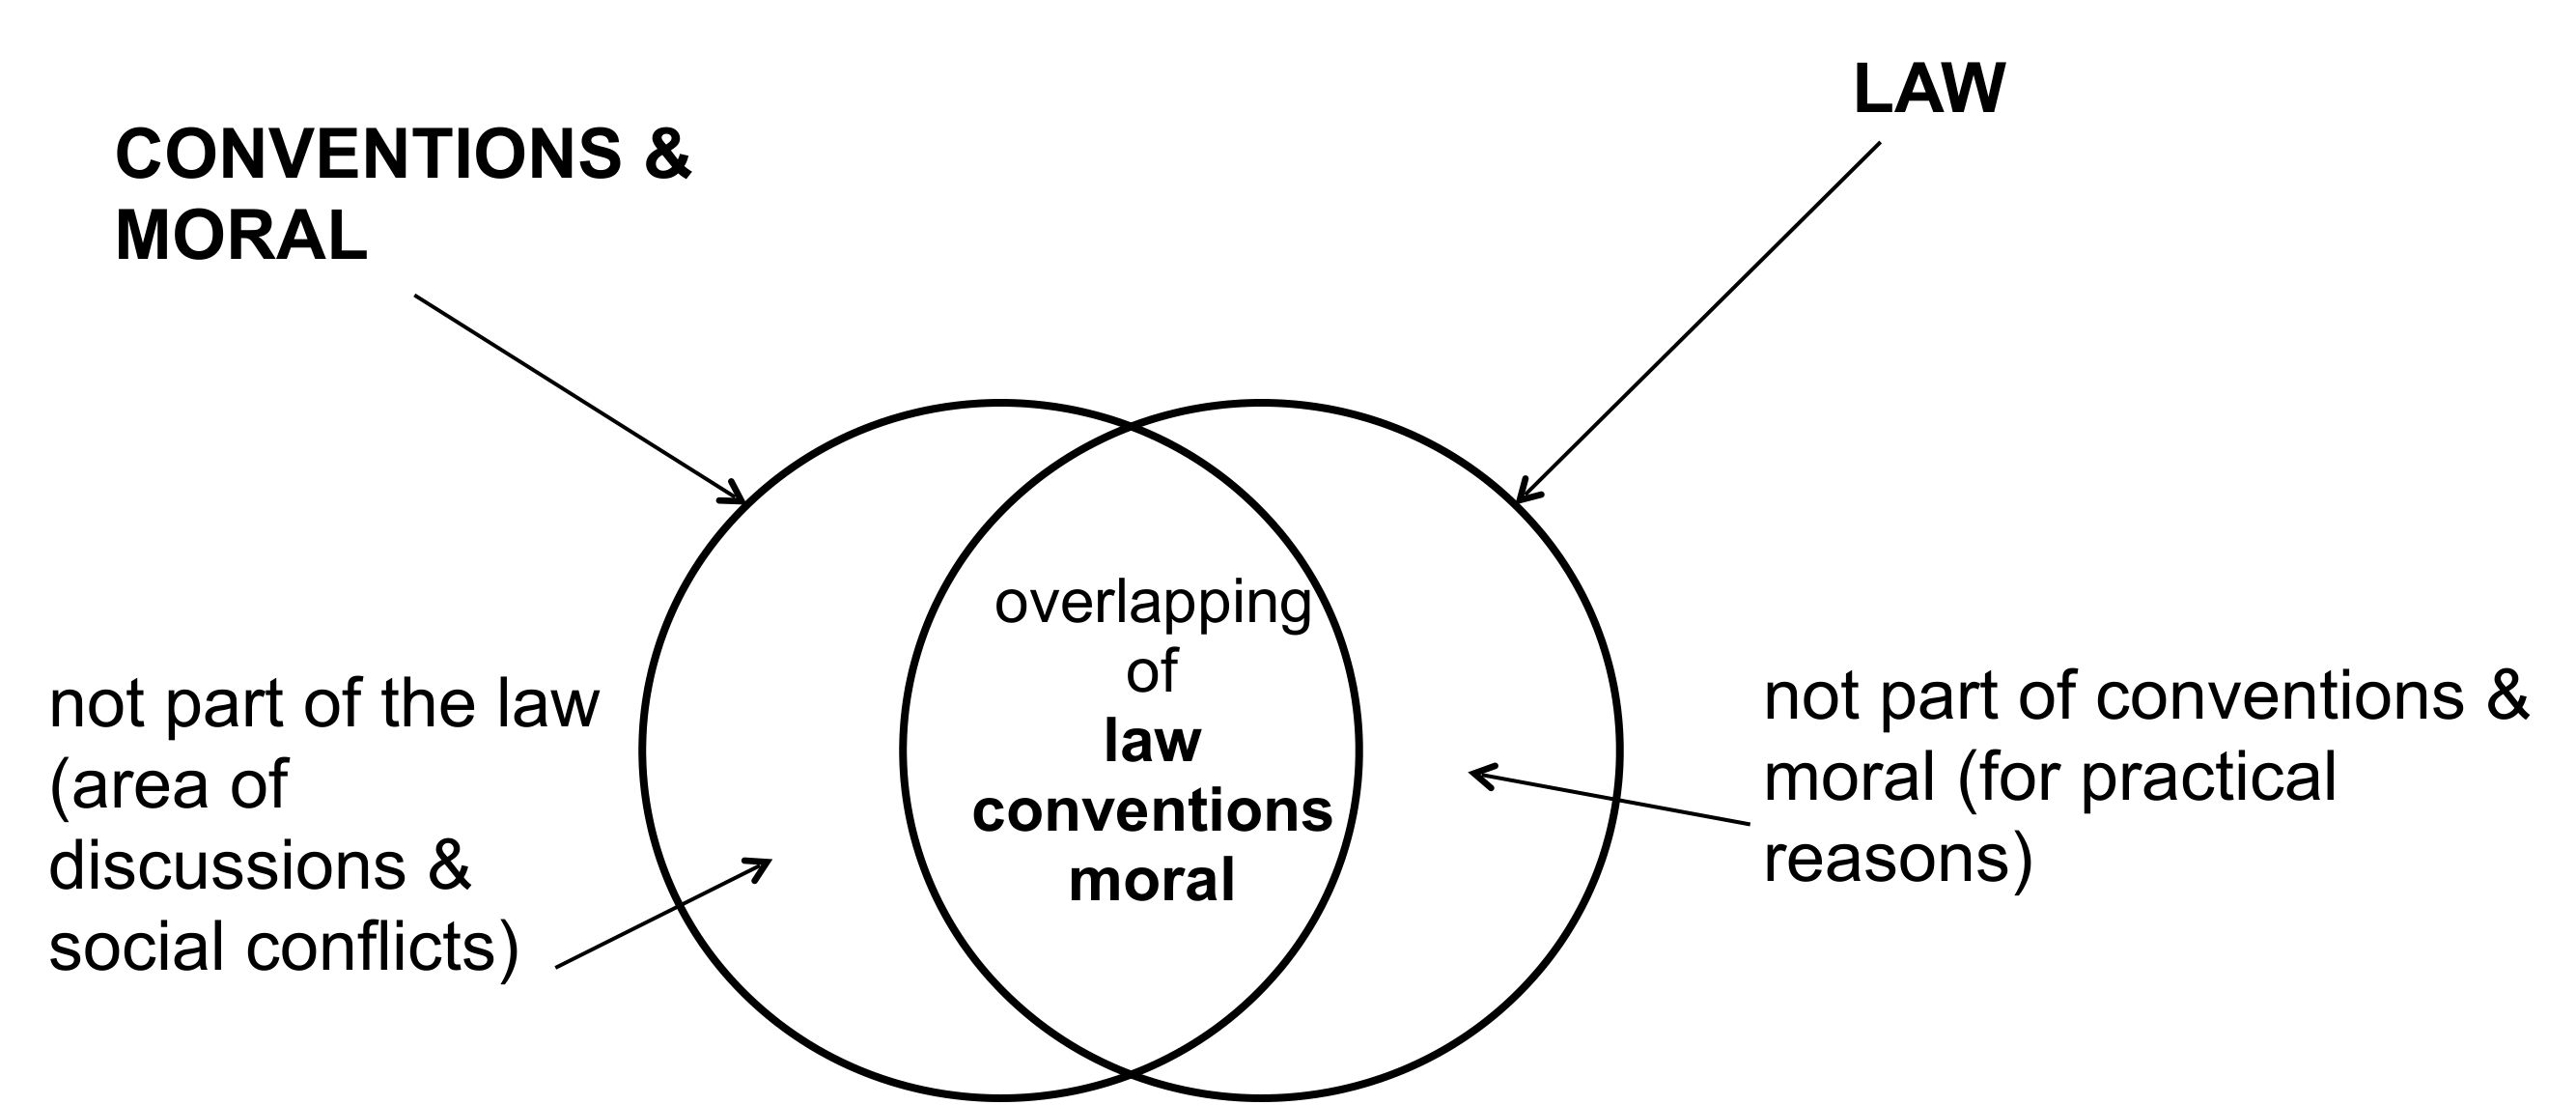
\includegraphics[width=0.8\linewidth]{img/conventions_moral_law}
	\caption{The relationship between conventions, morals and law}
	\label{fig:conventionsmorallaw}
\end{figure}

\subsection{Correct Legal Argumentation}
A statement or claim has to be justified by legal articles or arguments and the necessary evidence. Or is based on legal articles or arguments and with the necessary evidence arrives at a conclusion.

The law get classified by
\begin{itemize}
	\item Status: constitution, act, regulations or by-law
	\item Issuer: Federal, Cantonal and Communal Law
	\item Source of the Law: written law, common law, judicial tradition
	\item Involved Person: Civil Law or Public Law
\end{itemize}

At each of the federal, cantonal and communal level there is a separation of power into the \textbf{legislative}, the \textbf{executive} and the \textbf{Judiciary}, which provides a check and balance on the power of each authority.

\subsection{State, Cantons, Communes}

"Das Schweizervolk und die Kantone [...] bilden die Schweizerische Eidgenossenschaft", (1. Art BV).

"Der Kanton arbeitet mit den Gemeinden, den anderen Kantonen, dem Bund und, in seinem Zuständigkeitsbereich, mit dem Ausland zusammen." Therefore the State is only entitled to legislate and act in a territory or legal field where it has a constitutional legitimacy. The cantons are superior to the state in their power of legislation.

\begin{center}
	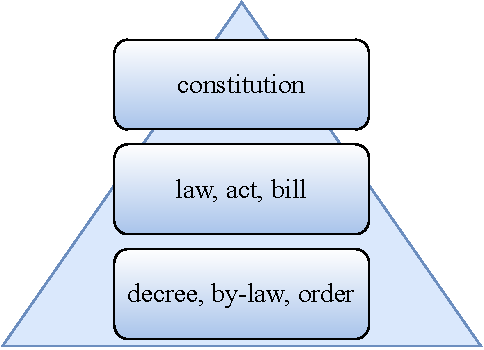
\includegraphics[width=0.4\linewidth,keepaspectratio]{law_hierarchy}
\end{center}

\begin{tabularx}{\linewidth}{X|X}
	\textbf{civil law} & \textbf{public law}\\
	\hline
	OR/ZGB & StGB\\
	GeBüV & FMG\\
	DSG & BÜPF/VÜPF\\
	URG, UWG & EIDI-V\\
	\vdots & \vdots
\end{tabularx}

Civil law is mastered by the \textbf{principle of freedom} of coalition and freedom of contract. Public law is mastered by the \textbf{principle of legality}, the control of power. This results in completely different jurisdictions with different procedures and rights for each.

\subsection{By-Law (Verordnung) $\neq$ Order (Verfügung)}

A By-Law is a \textbf{general, abstract regulation} as part of a law, while an order is an \textbf{individual, concrete application} of a law to a person.

\subsection{Legal Terms}
\begin{itemize}
	\item mandatory rules, stipulated rules and dispositive rules
	\item bona fide or good faith (ZGB 2)
	\item acting in good faith or a fair manner
	\item judicial discretion (ZGB 4)
	\item burden of proof (ZGB 8)
\end{itemize}

\subsection{International Law Framework}
Switzerland is integrated into the European legal framework by long-time traditions, unilateral and bilateral conventions. The IPRG ("Gesetz über das internationale Privatrecht") specifies the bridge between Swiss and foreign law. It rules which law is applicable and which court is competent. Parties can decide in most cases, under which jurisdiction they want to handle their disputes and which court will be competent.

There are generally three different instances in these jurisdictions:
\begin{itemize}
	\item Bezirksgericht
	\item Kantonsgericht
	\item Bundesgericht
\end{itemize}

\section{Copyright}
Through applying creative intellect a work is created. This work enjoys copyright, which means the creator may decide how this work is distributed. Copyright law guarantees them financial remuneration for the utilisation of their works. Moreover, the copyright law protects artists’ intellectual property in that they are able to defend themselves against
misappropriation of their work. Creative endeavour is a public good. Intellectual creations are the driving force of our economy.

\subsection{Prerequisites for Legal Protection of a Work}
A work must be an \textbf{intellectual creation} and have \textbf{Statistical Uniqueness}:
\begin{itemize}
	\item Individual character, characteristic features
	\item Sufficiently creative step, work is special and unique
\end{itemize}

There must be a perceptibility or expression of an idea. And ultimately a work must be created by humans.

With the new law all photographs and reproductions produced by similar methods of three-dimensional objects (film stills) will be subject to copyright protection.

\paragraph{Art 3 Swiss Copyright Act - Derivative Works}
\begin{enumerate}[label=\arabic* ]
	\item Derivative works are intellectual creations with an individual character that are \textbf{based upon pre-existing works, whereby the individual character of the latter remains identifiable.}
	\item Such works include, in particular, \textbf{translations} as well as audio-visual and other \textbf{adaptations}.
	\item Derivative works are protected as \textbf{works in their own right}.
	\item The protection of the works used in the derivative work remains reserved.
\end{enumerate}

To create a derivative work you require the consent of the copyright owner of the original work.

\subsection{Non-derivative Works}
\begin{enumerate}[label=\arabic* ]
	\item \textbf{rework}
	\begin{itemize}
		\item use of pre-existing works
		\item mere rework of an original work, no individual character
	\end{itemize}
	\item \textbf{new creation}
	\begin{itemize}
		\item original work is merely an inspiration and cannot be recognised or identified in the new creation
		\item the newly created work is protected individually in its own right
	\end{itemize}
\end{enumerate}

\subsection{Meaning of Copyright}
The \textbf{author of a copyrighted work} is always the natural person who created the work, which is known as \textbf{creator principle}.	Copyright law is an \textbf{absolute right} and thus excludes every other person. Copyrights can be transferred from the \textbf{original author} to another person or legal entity who then becomes the \textbf{right holder}.

\paragraph{Art 9 Swiss Copyright Act}
\begin{enumerate}[label=\arabic*]
	\item The author has the exclusive right to his own work and the right to recognition of his authorship.
	\item The author has the exclusive right to decide whether, when, how and under what author's designation his own work is published for the first time.
	\item A work is considered to be published when it has been made available for the first time by the author, or with his consent, to a large number of persons not constituting a private circle.
\end{enumerate}

\paragraph{Art 10 Swiss Copyright Act}
\begin{enumerate}[label=\arabic*]
	\item \textbf{The author has the exclusive right to decide whether, when and how his work is used.}
	\item The author has the right, in particular:
	\begin{enumerate}[label=\alph*.]
		\item to produce \textbf{copies} of the work, such as printed matter, phonograms, audio-visual fixations or data carriers;
		\item to offer, transfer or otherwise \textbf{distribute} copies of the work;
		\item to recite, \textbf{perform} or present a work, or make it \textbf{perceptible} somewhere else or \textbf{make it available} directly or through any kind of medium in such a way that persons may access it from a place and at a time individually chosen by them;
		\item to \textbf{broadcast} the work by radio, television or similar means, including by wire;
		\item to \textbf{retransmit} works by means of technical equipment, the provider of which is not the original broadcasting organisation, in particular including by wire;
		\item to make works made available, broadcast and retransmitted \textbf{perceptible}.
	\end{enumerate}
	\item The author of a computer program also has the exclusive rental right.
\end{enumerate}

\paragraph{Art 11 Swiss Copyright Act}
\begin{enumerate}[label=\arabic*]
	\item The author has the exclusive right to decide:
	\begin{enumerate}[label=\alph*.]
		\item whether, when and how the work may be \textbf{altered};
		\item whether, when and how the work may be used to create a \textbf{derivative work} or may be \textbf{included in a collected work}.
	\end{enumerate}
	\item Even where a third party is authorised by contract or law to alter the work or to use it to create a derivative work, the author may \textbf{oppose any distortion} of the work that is a violation of his personal rights.
	\item It is permissible to use existing works for the creation of parodies or other comparable variations on the work.
\end{enumerate}

\paragraph{Art 15 Swiss Copyright Act}
\begin{enumerate}[label=\arabic*]
	\item Where the owner of an original work of which no further copies exist has reason to assume that the author of the work has a legitimate interest in its preservation, he may not destroy the work without first offering to return it to the author. The owner may not request more than the material value of the work.
\end{enumerate}

\subsection{Transfer of Copyright}
Moral rights vest in the author and cannot be transferred or licensed, but they may be waived or transferred to heirs upon death.

\textbf{Economic rights may be transferred to third parties and transferred to heirs upon death, use rights may be licensed.}

The transfer of a work or copy of the work does not transfer the rights in the work, even if the original work is transferred.

\subsection{Joint Authorship}
This happen when multiple people \textbf{work together} pursuant to a \textbf{common concept} to create a work together. They can decide jointly on what happens with the work and must all agree to that.

\subsection{Duration of Copyright}
In Switzerland there is an \textbf{automatic protection with no formalities required}. A work is protected under copyright as soon as it is \textbf{created}.

Copyright protection starts as soon as a work is created and the prerequisites
for protection are met. In Switzerland copyright protection expires \textbf{70 years after the death of the author}. The protection for \textbf{computer programs} ends \textbf{50 years after the death of the author}. The protection of \textbf{pictures which do not possess an individual character} ends \textbf{50 years after their creation}.

\subsection{Limitations of Copyright}
\begin{center}
	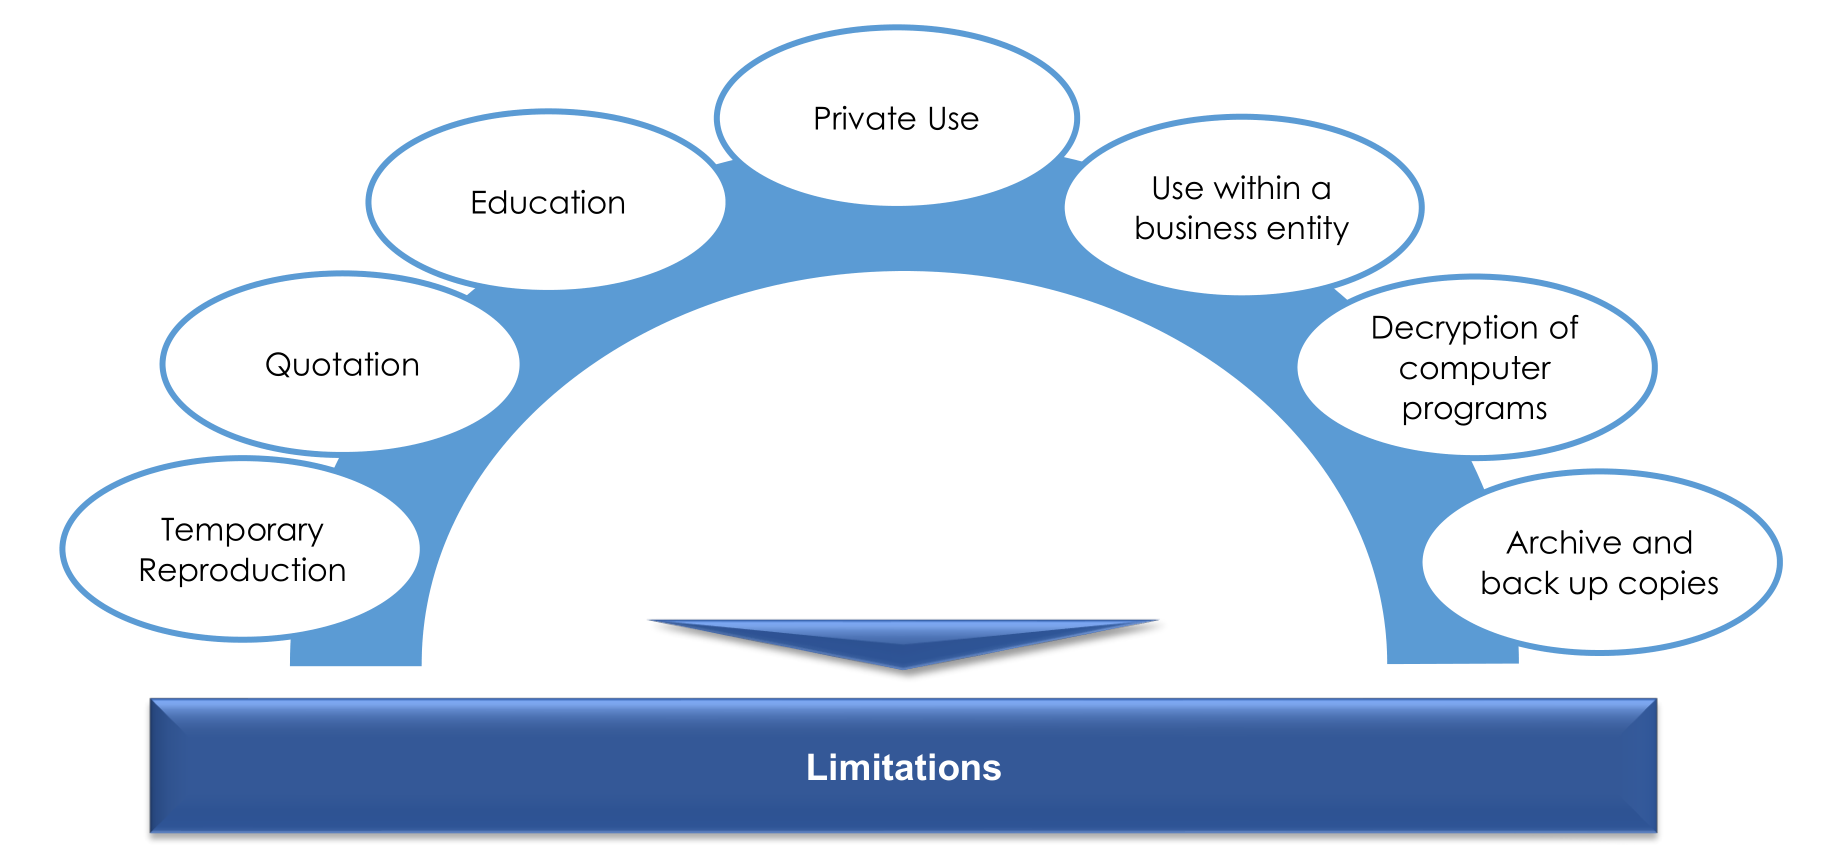
\includegraphics[width=0.8\linewidth]{img/limitations_of_copyright}
\end{center}
Private use includes only the \textbf{use in a private setting for private purposes},
sharing with family and close friends (private circle). \textbf{Private use is not subject to a license fee}. The download of copyrighted works is considered private use. 

\subsection{Related Rights}
The Copyright Act also regulates related rights also referred to as neighbouring rights.
\begin{itemize}[label=-]
	\item rights of \textbf{performing artists} to their performances
	\item rights of \textbf{producers of phonograms and videograms} to their products
	\item rights of \textbf{broadcasters} to their radio and television broadcasts
\end{itemize}

Related rights protection expires \textbf{50 years after the performance}, the publication of the phonogram or videogram or the production of it, in the case that it is not published or the emission of the broadcast.

\subsection{Civil Proceedings}
A copyright claim between private persons or private legal entities are discussed in civil proceedings in a civil court. The \textbf{right holder can request from the civil court}:
\begin{itemize}
	\item a declaratory judgement, that is have a right established
	\item have an infringement banned or remedied
	\item have property confiscated
	\item have an order published
	\item claim damages
\end{itemize}

\subsection{Criminal Proceedings}
% TODO Criminal Procedures

% TODO Collecting Societies

% TODO Copyright and the Internet

% TODO International Treaties







\end{document}
